\newtheorem{lemma}{Lemma}
\newtheorem{proof}{Proof}
\newtheorem{hpp_problem_basic}{Problem}

\section{HPP}
In this section we present the \textit{Learning a Parallelepiped} attack as described in \cite{NR09}. 
Note that in this section bold lowercase $\vec{v}$ denotes a \textit{row}-vector to follow the same notation as in the original paper.
\subsection{Setup and idealized version}
Let $\mat{V} \in \mathcal{GL}(\bb{R})$ be a secret $n \times n$ unimodular matrix and $\PP{V}$ be a fundamental parallelepiped, defined as the set $\{\vec{x}\mat{V}: \vec{x} \in [-1, 1]^n\}$. 
Let $\vec{v} = \vec{x} \mat{V}$. 
The problem to solve is informally described below and visualized in figure \ref{hpp_parallelepiped_uniform}.

\begin{hpp_problem_basic}\label{Basic HPP problem}
    Given enough vectors $\vec{v} = \vec{x}\mat{V}$ (i.e. by observing a large enough subset of $\PP{V}$), where both $\vec{x}$ and $\mat{V}$ is unknown,
recover rows of $\pm \mat{V}$
\end{hpp_problem_basic}
The following three steps are used to solve Problem \ref{Basic HPP problem}:
\begin{enumerate}
    \item Estimate the covariance matrix $\mat{V}^t \mat{V}$
    \item Transform samples $\vec{v} \in \PP{V}$ to $\vec{c} \in \PP{C}$ where $\PP{C}$ is a hypercube, i.e. $\mat{C} \mat{C}^t = \mat{I}_n$
    \item Do gradient descent to minimize the fourth moment of one-dimensional projections and reveal a row of $\pm \mat{C}$ which finally can be transformed into a row of $\pm \mat{V}$
\end{enumerate}
In the following, each of these steps will be covered in detail.
\begin{figure}[H]
    \centering
    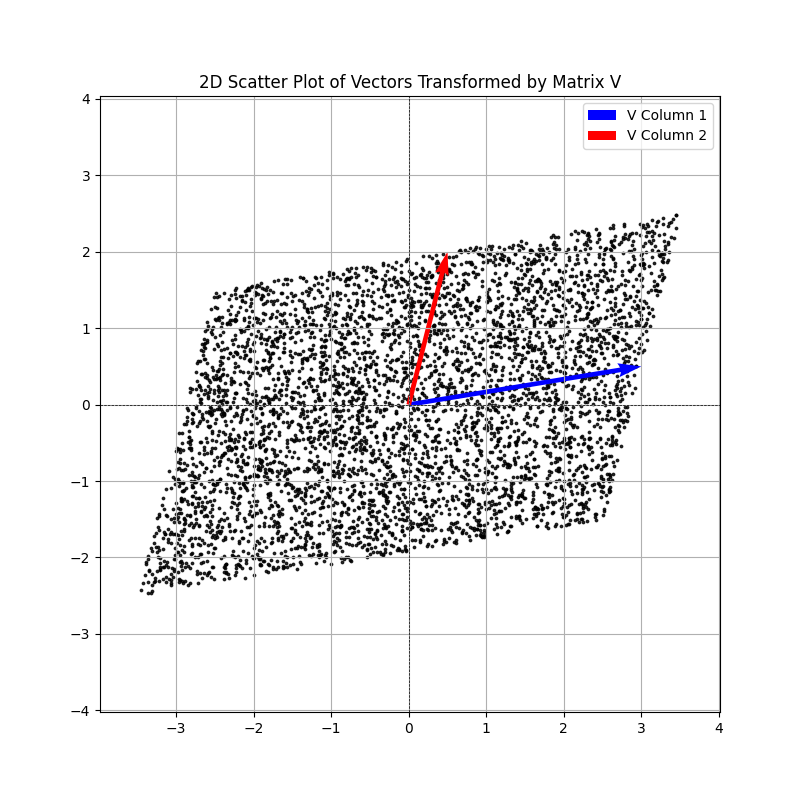
\includegraphics[scale=0.5]{hpp_parallelepiped_uniform.png}
    \caption{Hidden parallelepiped problem in dimension 2. Given only signature samples, recover rows of $\mat{V}$, here marked as vectors in red and blue}
  	\medskip 
	% \hspace*{15pt}\hbox{\scriptsize Credit: Acme company makes everything \url{https://acme.com/}}
    \label{hpp_parallelepiped_uniform}
\end{figure}
\subsection{Covariance matrix estimation}
Given enough samples on the form $\vec{v} = \vec{x}\mat{V} $, we want to estimate the covariance matrix $\mat{G} \approx \mat{V}^t \mat{V}$.
This is achieved as $\vec{v}^t \vec{v} = ( \vec{x}\mat{V})^t(\vec{x}\mat{V}) = \mat{V}^t \vec{x}^t \vec{x} \mat{V}$.
% Remark that since $\vec{x}$ is a row vector, $\bb{E}[\vec{x}^t \vec{x}]$ will be an $n \times n$ matrix.
Now, by taking the expectation of the inner term we get $\bb{E}[\vec{x}^t \vec{x}] = \mat{I}_n / 3$ where $\mat{I}_n$ is the $n \times n$ identity matrix because of the following:
Since all $x_i \in \vec{x}$ are distributed according to the uniform distribution over $[-1, 1]$ and each $x_i$ are independent, 
we have that $\bb{E}[x_i] = 0$ and $\bb{E}[x_i x_j] = \bb{E}[x_i] \bb{E}[x_j] = 0$ when $i \neq j$.
For the case when $i = j$, we have 

\[\bb{E}[x_i x_j] = \bb{E}[x ^2] = \int_{a}^{b} x^2 \frac{1}{b-a} dx = \int_{-1}^{1} x^2 \frac{1}{2} dx = \frac{1}{3}\]

Therefore, $\bb{E}[\vec{x}^t \vec{x}]$ is an $n \times n$ matrix with $\mathlarger{\frac{1}{3}}$ down the diagonal and is 0 otherwise, i.e. $\mat{I}_n / 3$.
Thus, as number of samples grow, $\vec{v} ^t \vec{v} \rightarrow \mat{V}^t (\mat{I}_n / 3) \mat{V}$, and therefore $\vec{v}^t \vec{v} \cdot 3 \rightarrow \mat{V}^t \mat{V}$.
In conclusion: by taking the average of $\vec{v}^t \vec{v}$ for all collected samples, and multiplying the resulting $n \times n$ matrix with $3$, one 
has a good approximation of the covariance matrix $\vec{V}^t \vec{V}$.
% Clearly, the more samples $\vec{v}$ one has, the more accurate the approximation $\mat{G} \approx \mat{V} ^t \mat{V}$ is.
\subsection{Hidden parallelepiped to hidden hypercube transformation}
Given a good approximation $\mat{G} \approx \mat{V}^t \mat{V}$, the next step is to calculate a linear transformation $\mat{L}$ such that the following is true:
\begin{enumerate}
    \item $\mat{C} = \mat{V}\mat{L}$ is orthonormal, i.e. the rows are pairwise orthogonal and the norm of each row is 1. In other words, $\mat{C} \mat{C}^t = \mat{I}$. 
        Consequently, $\PP{C}$ becomes a hypercube.
    \item If $\vec{v}$ is uniformly distributed over $\PP{V}$ then $\vec{c} = \vec{v} \mat{L}$ is uniformly distributed over $\PP{C}$.
\end{enumerate}
% This transformation is visualized from figure \ref{hpp_parallelepiped_uniform} to figure \ref{hpp_uniform_cube}.
This is achieved by taking the Cholesky decomposition of $\mat{G}^{-1} = \mat{L} \mat{L}^t$ where $\mat{L}$ is a lower-triangular matrix. 
To compute Cholesky decomposition of $\mat{G}^{-1}$, we must first show that $\mat{G}$ is symmetric positive definite.
\begin{enumerate}
    \item $\mat{G}$ is symmetric $\iff \mat{G}^{t}= \mat{G}$ which is clear as $\mat{G}^t = (\mat{V}^t\mat{V})^t = \mat{V}^t (\mat{V}^{t})^t= \mat{V}^t \mat{V} = \mat{G}$.
    \item $\mat{G}$ is positive definite if for any non-zero column vector $\vec{x} \in \bb{R}^n$, $\vec{x}^t \mat{G} \vec{x} > 0.$
We have that $\vec{x}^t \mat{G} \vec{x} = \vec{x}^t \mat{V}^t \mat{V} \vec{x} = (\mat{V} \vec{x})^t (\mat{V} \vec{x})$. Denote by $\vec{y} = \mat{V} \vec{x}$.
Since $\vec{x} \neq \mathbf{0}$ and $\mat{V}$ is invertible (and therefore non-zero) it is clear that 
$\vec{y} \neq \mathbf{0}$ and $\vec{y}^t \vec{y} = \lvert \vert{\vec{y}} \rvert \vert ^2 > 0$.
\end{enumerate}
Since $\mat{G}$ is symmetric positive definite we can do decomposition to get $\mat{L}$. Then: 
\begin{enumerate}
    \item if $\mat{C} = \mat{V} \mat{L}$, then $\mat{C} \mat{C}^t = \mat{V} \mat{L} \mat{L}^t \mat{V}^t = \mat{V} \mat{G}^{-1} \mat{V}^t = \mat{V} (\mat{V^t}\mat{V})^{-1} \mat{V}^t
        = \mat{V} \mat{V}^{-1} \mat{V}^{-t} \mat{V}^t = \mat{I}$
    \item since entries in $\vec{v} = \vec{x} \mat{V}$ is uniformly distributed over $\PP{V}$, $\vec{c} = \mat{C} \vec{x}$ is uniformly distributed over $\PP{C}$
\end{enumerate}

By multiplying our samples $\vec{v}$ by $\mat{L}$ on the right, we transform them from the hidden parallelepiped to the hidden hypercube. 
Therefore, the problem to solve now can be called the "Hidden Hypercube Problem".
If one finds the rows of $\pm \mat{C}$, one can simply multiply the result on the right by $\mat{L}^{-1}$ to obtain the solution for $\mat{V}$.

\begin{figure}[H]
    \centering
    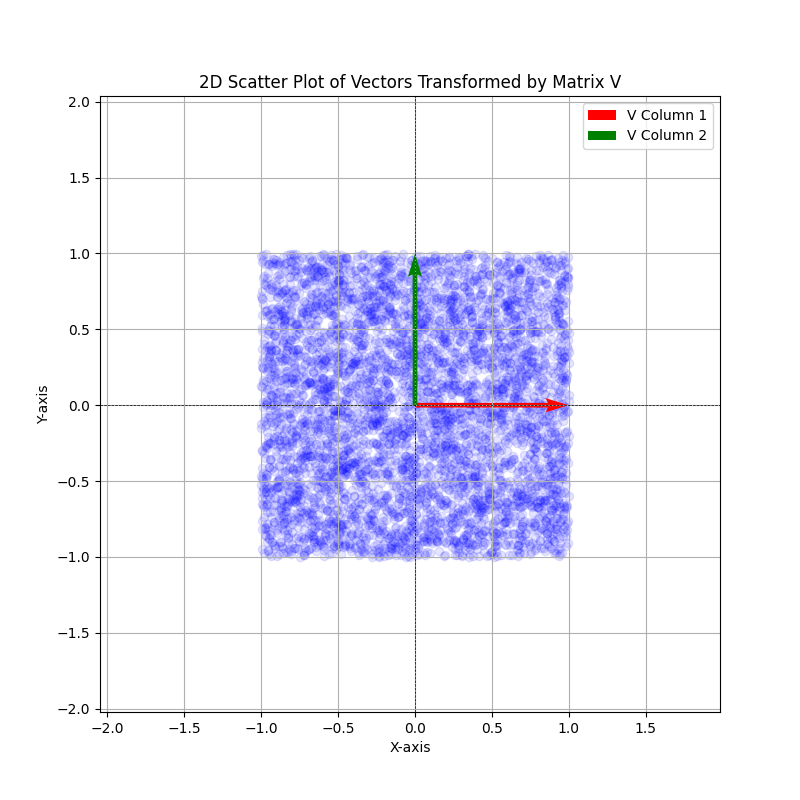
\includegraphics[scale=0.5]{hpp_uniform_cube.png}
    \caption{Hidden hypercube problem in dimension 2}
  	\medskip 
	% \hspace*{15pt}\hbox{\scriptsize Credit: Acme company makes everything \url{https://acme.com/}}
    \label{hpp_uniform_cube}
\end{figure}
\subsection{Moments and Gradient Descent}
The last major step in the attack is to measure and minimize the fourth moment of one-dimensional projections to disclose rows of $\pm \mat{C}$.
Let $mom_{k, \mat{C}}(\vec{w})$ be defined as the $k$-th moment of $\PP{C}$ projected onto $\vec{w}$, i.e. 
$\bb{E}[\langle \vec{c}, \vec{w} \rangle ^k]$ where $\vec{c} = \vec{x} \mat{C}$ for $\vec{x}$ uniformly distributed and $\vec{w} \in \bb{R}^n$.
Looking at the term $\langle \vec{c}, \vec{w} \rangle$, we have $\langle \vec{x} \mat{C}, \vec{w} \rangle = \langle \sum_{i=1}^{n} x_i c_i, \vec{w} \rangle$
where $c_i$ is the $i$-th row of $\mat{C}$. Since $x_i$ is a scalar, we can move it out of the dot-product brackets as $\sum_{i=1}^{n} x_i \langle c_i, \vec{w} \rangle $ .
Evaluating this inside the expectation operator $\bb{E}[ \ ]$ we have $\bb{E}[\sum_{i=1}^{n} x_i \langle c_i, \vec{w} \rangle ^k ]$.
We consider the two cases when $k = 2$ and $k=4$.
\begin{itemize}
    \item $\mathbf{k = 2: }$
        $\bb{E}[(\sum_{i=1}^{n} x_i \langle c_i, \vec{w} \rangle ) ^2] \text{ expands to } \bb{E}[\sum_{i}^{n} \sum_{j}^{n} x_i x_j \langle c_i, \vec{w} \rangle \langle c_j, \vec{w} \rangle]$.
        As seen before in section 3.4.2, $\bb{E}[x_i x_j] = \frac{1}{3}$ when $i = j$ and $0$ otherwise. Thus, we have the expression 
        $mom_{2, C}(\vec{w}) = \frac{1}{3} \sum_{i}^{n} \langle c_i, \vec{w} \rangle ^2$ which can also be written as
        $ = \frac{1}{3} \vec{w} \mat{C}^t \mat{C} \vec{w}^t$ \todo{Should show why this is}

    \item $\mathbf{k = 4: }$
        \[ \bb{E}[(\sum_{i=1}^{n} x_i \langle c_i, \vec{w} \rangle ) ^4] = 
        \bb{E}[\sum_{i}^{n} \sum_{j}^{n} \sum_{k}^{n} \sum_{l}^{n} x_i x_j x_k x_l 
        \langle c_i, \vec{w} \rangle \langle c_j, \vec{w} \rangle
    \langle c_k, \vec{w} \rangle \langle c_l, \vec{w} \rangle] \]
    There are three cases for the indices $i, j, k$ and $l$:
    \begin{enumerate}
        \item \textbf{All equal: } If $i = j = k = l$, we simply have $\sum_i^n \bb{E}[x^4] \langle c_i, \vec{w} \rangle ^4 = \frac{1}{5} \sum_i \langle c_i, \vec{w} \rangle ^4$
            due to the fact that $\bb{E}[x ^4] = \int_{-1}^{1} x^4 \frac{1}{2} dx = \frac{1}{5}$
        \item \textbf{None equal:} If $i \neq j \neq k \neq l$ the expression is zero due to $\bb{E}[x_i] = 0$ and all $x_i, x_j, x_k, x_l$ are independent.
        \item \textbf{Pairwise equal:} If either 
            \begin{itemize}
                \item $i = j \neq k = l$
                \item $i = k \neq j = l$ 
                \item $i = l \neq j = k$
            \end{itemize}
            then we have 
            $\sum_{i \neq j} \bb{E}[x_i ^2 x_j^2] \langle c_i, \vec{w} \rangle ^2 \langle c_j, \vec{w} \rangle^2$ 
            $ = \frac{1}{9} \sum_{i \neq j} \langle c_i, \vec{w} \rangle^2 \langle c_j, \vec{w} \rangle^2$. By putting the above together we get
            \[\frac{1}{5} \sum_{i=1}^{n} \langle c_i, \vec{w} \rangle ^4 + 3(\frac{1}{9} \sum_{i \neq j} \langle c_i, \vec{w} \rangle ^2 \langle c_j, \vec{w} \rangle ^2)\]
            and the final expression becomes 
            \[ mom_{4, \mat{C}} (\vec{w}) = \frac{1}{5} \sum_{i=1}^{n} \langle c_i, \vec{w} \rangle ^4 + \frac{1}{3} \sum_{i \neq j} \langle c_i, \vec{w} \rangle ^2 \langle c_j, \vec{w} \rangle ^2\]
    \end{enumerate}
    \end{itemize}

Now, since $\mat{C}$ is orthonormal, and by restricting $\vec{w}$ to the unit sphere in $\bb{R}^n$, we can simplify the expressions further.
The second moment becomes $mom_{2, C}(\vec{w}) = \frac{1}{3} \vec{w} \mat{C}^t \mat{C} \vec{w}^t = \frac{1}{3}\vec{w} \mat{I} \vec{w}^t 
= \frac{1}{3} \vec{w}\vec{w}^t = \frac{1}{3} \lVert \vec{w} \rVert ^2 = \frac{1}{3}$. 

By rewriting and expanding the fourth moment:
\[ mom_{4, \mat{C}} (\vec{w}) = \frac{1}{5} \sum_{i=1}^{n} \langle c_i, \vec{w} \rangle ^4 + \frac{1}{3} \sum_{i \neq j} \langle c_i, \vec{w} \rangle ^2 \langle c_j, \vec{w} \rangle ^2\]
\[ mom_{4, \mat{C}} (\vec{w}) = \frac{1}{5} \sum_{i=1}^{n} \langle c_i, \vec{w} \rangle ^4 + 
    \frac{1}{3} \sum_{i=1}^{n} \sum_{j=1}^n \langle c_i, \vec{w} \rangle ^2 \langle c_j, \vec{w} \rangle ^2 -
\frac{1}{3}\sum_{i=1}^{n} \langle c_i, \vec{w} \rangle ^2 \langle c_i, \vec{w} \rangle ^2\]
\[ mom_{4, \mat{C}} (\vec{w}) = \frac{1}{5} \sum_{i=1}^{n} \langle c_i, \vec{w} \rangle ^4 + 
\frac{1}{3} \sum_{i=1}^n \sum_{j=1}^n \langle c_i, \vec{w} \rangle ^2 \langle c_j, \vec{w} \rangle ^2 -
\frac{1}{3}\sum_{i=1}^{n} \langle c_i, \vec{w} \rangle ^4 \]
\[ mom_{4, \mat{C}} (\vec{w}) = \frac{1}{3} \lVert \vec{w} \rVert ^4 - 
    \frac{2}{15}\sum_{i=1}^{n} \langle c_i, \vec{w} \rangle ^4 = \frac{1}{3} - 
\frac{2}{15}\sum_{i=1}^n \langle c_i, \vec{w} \rangle ^4\]


The key observation is that to minimize $mom_{4, \mat{C}(\vec{w})}$ one has to maximize the term 
$ \mathlarger{-\frac{2}{15}\sum_{i=1}^{n}} \langle c_i, \vec{w} \rangle ^4$. Since $c_i$ and $\vec{w}$ are both on the unit circle, and
all $c_i$ are orthogonal to each other, the term is maximized whenever $\vec{w} = c_i$ since $\langle c_i, \pm c_i \rangle = \langle \vec{w}, \pm \vec{w} \rangle = 1$.
Using this observation, we employ a gradient descent to minimize $mom_{4, \mat{C}}(\vec{w})$ w.r.t the input vector $\vec{w}$, and the global minima is in $\pm \mat{C}$.
The expression when $\vec{w} = \pm c_i$ is 
\[
    % mom_{4, \mat{C}}(\pm c_i) = \frac{1}{3} - \frac{2}{15} \mathlager{\sum_{i=1}^{n} \langle c_i, \pm c_i \rangle ^4}
    % = \frac{1}{3} - \frac{2}{15} = \frac{1}{5}
    mom_{4, \mat{C}}(\pm c_i) = \frac{1}{3} - \frac{2}{15} \mathlarger{\sum_{i=1}^{n}} \langle c_i, \pm c_i \rangle ^4
    = \frac{1}{3} - \frac{2}{15} = \frac{1}{5}
\]

To do a gradient descent we need to compute the gradient of the fourth moment, $\nabla mom_{4, \mat{C}} (\vec{w})$.
\begin{itemize}
    \item The gradient of the first term, $\frac{1}{3} \lVert \vec{w} \rVert ^4$, is computed as follows: \\
        We rewrite $\lVert \vec{w} \rVert ^4$ as $(\vec{w}\vec{w}^T)^2$. Using the chain rule we have that \\
        $\nabla ((\vec{w}\vec{w}^T)^2) = 2(\vec{w}\vec{w}^T) \cdot \frac{\partial}{\partial \vec{w}_j}(\vec{w}\vec{w}^T)$
        $= 2(\vec{w}\vec{w}^T) \cdot 2 \vec{w}$. \\ 
        The gradient of the first term is then $\frac{1}{3} \cdot 2(\vec{w}\vec{w}^T) \cdot 2 \vec{w} = \frac{4}{3} \lVert \vec{w} \rVert ^2 \vec{w}$.
    \item For the second term, $\frac{2}{15} \mathlarger{\sum_{i=1}^{n} \langle c_i, \vec{w} \rangle ^4}$ we use the fact that the gradient is a linear operator:
        \[\nabla \sum_{i=1}^{n}\langle c_i, \vec{w} \rangle ^4 = \sum_{i=1}^{n}\nabla (\langle c_i, \vec{w} \rangle ^4)\]
        Looking at just the inner term, $\nabla (\langle c_i, \vec{w} \rangle ^4) = 4 \langle c_i, \vec{w} \rangle ^3 
        \cdot \frac{\partial}{\partial w_j} (\langle c_i, \vec{w} \rangle) = 4 \langle c_i, \vec{w} \rangle ^3 \cdot c_i$
        The gradient of the second term is therefore $\mathlarger{\frac{8}{15} \sum_{i=1}^{n} \langle c_i, \vec{w} \rangle ^3 c_i}$
\end{itemize}
Putting together the terms we get
\[ \nabla mom_{4, \mat{C}}(\vec{w}) =  \frac{4}{3} \lVert \vec{w} \rVert ^2 \vec{w} - \frac{8}{15} \sum_{i=1}^{n} \langle c_i, \vec{w} \rangle ^3 c_i\]

\todo{Should prove that there are no other local minima somehow}

In a practical attack, one simply approximates $mom_{4, \mat{C}}(\vec{w})$ as $\bb{E}[\langle \vec{c}, \vec{w} \rangle ^4]$ by averaging over all available samples $\vec{c}$.
Similarly, to approximate the gradient of the 4th moment, $\nabla mom_{4, \mat{C}}(\vec{w})$, again, using the linearity of the gradient operator, 
we can compute $\bb{E} [\nabla \langle \vec{c}, \vec{w} \rangle ^4] = \bb{E} [4 \langle \vec{c}, \vec{w} \rangle ^3 \vec{c}] = 4 \bb{E} [\langle \vec{c}, \vec{w} \rangle ^3 \vec{c}]$
by averaging the expression over all available samples $\vec{c}$.

% Now that the gradient of $mom_{4, \mat{C}}(\vec{w})$ is well-defined, we continue with the gradient descent.
In Algorithm \ref{HPPGradientDescentAlg}, a simple gradient descent for minimization of $mom_{4, \mat{C}}(\vec{w})$ is described.
\begin{algorithm}
    \caption{Gradient descent}\label{HPPGradientDescentAlg}
\begin{algorithmic}[1]
% \Procedure{Euclid}{$a,b$}\Comment{The g.c.d. of a and b}
    \Require{Parameter $\delta$, samples $\vec{c}$}
        \State Choose random vector $\vec{w}$ on the unit sphere
        \State Compute an approximation $\vec{g} \gets \nabla mom_{4, \mat{C}}(\vec{w})$
        \State Set $\vec{w}_{new} \gets \vec{w} - \delta \vec{g} $
        \State Normalize $\vec{w}_{new}$ as $\frac{\vec{w}_{new}}{\lVert \vec{w}_{new} \rVert}$
        \State Approximate $mom_{4, \mat{C}}(\vec{w})$ and $mom_{4, \mat{C}}(\vec{w}_{new})$
        \If{$mom_{4, \mat{C}}(\vec{w}) \geq mom_{4, \mat{C}}(\vec{w}_{new})$}
            \State Return $\vec{w}$
        \Else{}
        \State Set $\vec{w} \gets \vec{w}_{new}$ and go to step 2
        \EndIf
\end{algorithmic}
\end{algorithm}
One such descent will return one a candidate row $c_i$ of $\pm \mat{C}$ that is a minimum in the gradient landscape.
By multiplying this row with $\mat{L}^{-1}$ on the right and rounding the entries one has a candidate row $v_i$ in $\pm \mat{V}$.
This procedure can be repeated until all rows of $\pm \mat{C}$ are found. 

Depending on the specific signature scheme one attacks, knowing when
all correct rows have been found can be a tricky task. For example, if all rows of $\mat{C}$ are independent of each other, one 
has to find the correct combination of the rows that constitutes $\mat{C}$. This requires at most $2 \cdot n!$ attempts, which quickly becomes an impossibly large number as $n$ grows. 
In the case of NTRU-sign, however, the rows are not independent. In fact, finding any \textit{one} single row of $\mat{C}$ reveals all the remaining rows,
up to a polynomial number of different ordered permutations. Thus, one successful descent effectively breaks the scheme.

\todo{Discuss the attack in practice, i.e. the attack against discrete uniform distribution etc.}

\section{HPP against a non-uniform distribution}
The success of the HPP attack is in part based on the assumption of an underlying uniform distribution of the vector $\vec{x}$.
We now investigate how the method would work against a different underlying distribution.

Assume now that observed signatures are on the form $\vec{c} = \vec{x} \mat{V}$ where $x_i \sim \mathcal{D}(0, \sigma)$, i.e. some distribution with expectation 0 and some standard deviance $\sigma$.
For this theoretical work we assume the distribution $\mathcal{D}(0, \sigma)$ is continuous as in the idealized version of HPP in section 3.4.

\section{HPP against normal distribution}
Assume now that the signatures on the form $\vec{v} = \vec{x} \mat{V}$ where $x_i \sim \normdist{0}{\sigma}$, the continuous normal distribution with $\mu = 0$ and std.dev. $\sigma$. 
After converting $\PP{V}$ to $\PP{C}$, the fourth moment of $\PP{C}$ is constant over $\vec{w}$ on the unit circle.

    To show this, we simply do the same calculations as in the previous section, with the difference that $x$ follows a normal distribution.
    Considering
    \[ mom_{4, \mat{C}}(\vec{w}) = \bb{E}[(\sum_{i=1}^{n} x_i \langle c_i, \vec{w} \rangle ) ^4] = 
        \bb{E}[\sum_{i}^{n} \sum_{j}^{n} \sum_{k}^{n} \sum_{l}^{n} x_i x_j x_k x_l 
        \langle c_i, \vec{w} \rangle \langle c_j, \vec{w} \rangle
    \langle c_k, \vec{w} \rangle \langle c_l, \vec{w} \rangle] \]

    for the three different cases:
    \begin{itemize}
        \item \textbf{All equal: } If $i = j = k = l$, we simply have $\sum_i^n \bb{E}[x_i^4] \langle c_i, \vec{w} \rangle ^4 = 3 \sigma ^4 \sum_i \langle c_i, \vec{w} \rangle ^4$
            due to the well known fact that $\bb{E}[x^4] = 3 \sigma ^4$ for $x$ distributed according to $\normdist{0}{\sigma}$.
        \item \textbf{None equal:} Since $\bb{E}[x] = 0$ and $x_i, x_j, x_k, x_l$ are independent, this results in zero.
        \item \textbf{Pairwise equal:} If either 
            \begin{itemize}
                \item $i = j \neq k = l$
                \item $i = k \neq j = l$ 
                \item $i = l \neq j = k$
            \end{itemize}
            we have $\sum_{i \neq j} \bb{E}[x_i^2 x_j^2] \langle c_i, \vec{w} \rangle ^2 \langle c_j, \vec{w} \rangle ^2$
            $= \sigma^4 \sum_{i \neq j}\langle c_i, \vec{w} \rangle ^2 \langle c_j, \vec{w} \rangle ^2$ since $\bb{E}[x^2] = \sigma^2$.
    \end{itemize}

    Putting together expressions like in section 3.4.4 we get 
    \[
        mom_{4, \mat{C}}(\vec{w}) = 3 \sigma ^4 \sum_i \langle c_i, \vec{w} \rangle ^4 + 3(\sigma^4 \sum_{i \neq j}\langle c_i, \vec{w} \rangle ^2 \langle c_j, \vec{w} \rangle ^2)
    \]
    \[
        mom_{4, \mat{C}}(\vec{w}) = 3 \sigma ^4 \sum_i \langle c_i, \vec{w} \rangle ^4 
        + 3\sigma^4 \sum_{i} \sum_{j} \langle c_i, \vec{w} \rangle ^2 \langle c_j, \vec{w} \rangle ^2
        - 3\sigma^4 \sum_{i} \langle c_i, \vec{w} \rangle ^4
    \]
    \[
        mom_{4, \mat{C}}(\vec{w}) = 3\sigma^4 \sum_{i} \sum_{j} \langle c_i, \vec{w} \rangle ^2 \langle c_j, \vec{w} \rangle ^2
    \]
    \[
        mom_{4, \mat{C}}(\vec{w}) = 3\sigma^4 (\lVert \vec{w} \rVert ^2 ) ^2 = 3 \sigma ^4
    \]

    Since $mom_{4, \mat{C}}(\vec{w})$ is constant for $\vec{w}$ on the unit sphere (depending only on $\sigma$), the term no longer depends on the secret matrix $\mat{C}$ and the attack will not work.

    \begin{figure}[H]
    \centering
    % \begin{minipage}{0.45\textwidth}
        \centering
        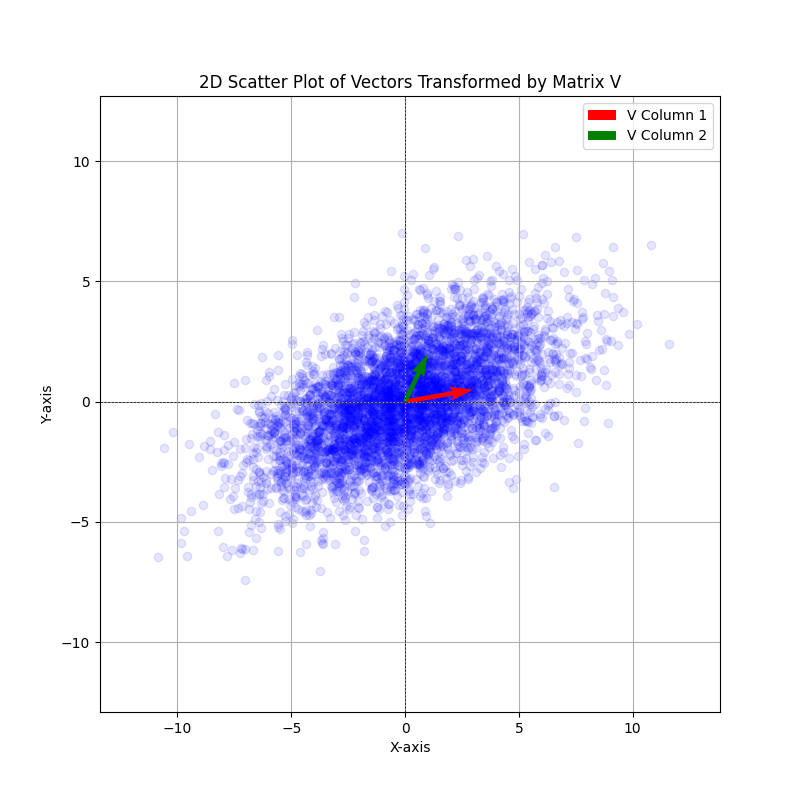
\includegraphics[width=0.9\textwidth]{hpp_parallelepiped_normal.png} % first figure itself
        \caption{HPP in dimension 2 for normal distribution}
        \medskip 
    % \end{minipage}\hfill
\end{figure}
\begin{figure}[H]
    % \begin{minipage}{0.45\textwidth}
        \centering
        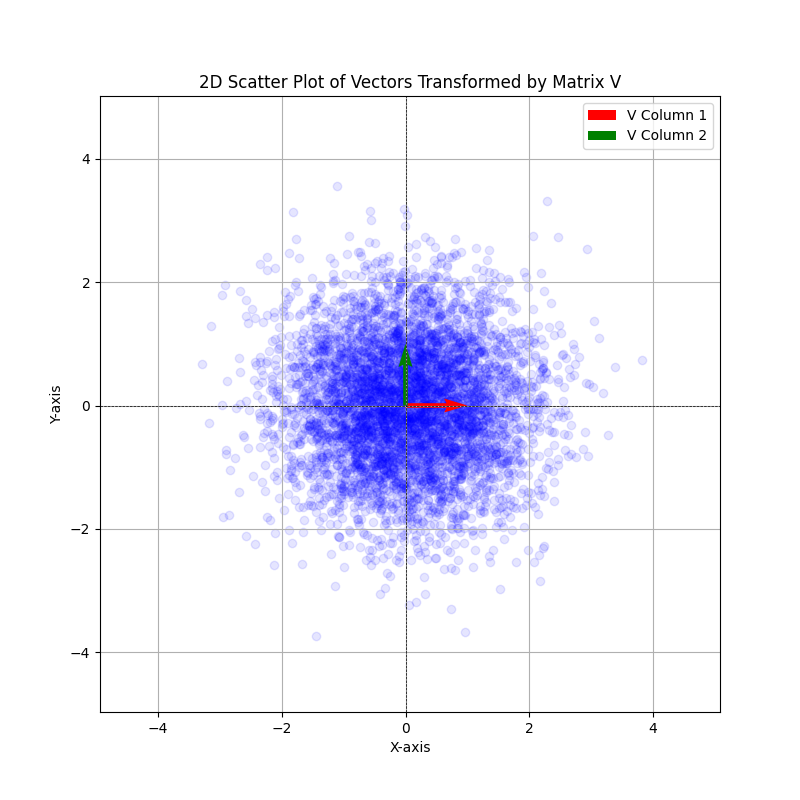
\includegraphics[width=0.9\textwidth]{hpp_normal_cube.png} % second figure itself
        \caption{Hidden hypercube problem in dimension 2 for normal distribution}
        \medskip 
    % \end{minipage}
\end{figure}
% \begin{figure}[H]
%     \centering
%     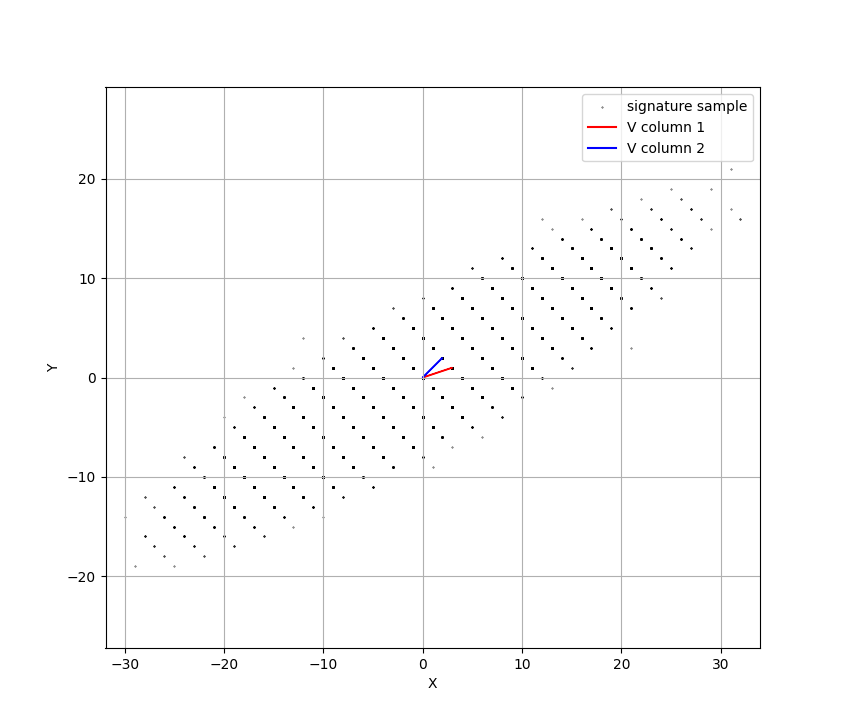
\includegraphics[scale=0.5]{hpp_parallelepiped_normal_discrete.png}
%     \caption{Hidden parallelepiped in dimension 2 for discrete Gaussian distribution ($\sigma = 2.02$)}
% 	% \hspace*{15pt}\hbox{\scriptsize Credit: Acme company makes everything \url{https://acme.com/}}
%     \label{parallelepiped_normal_discrete}
% \end{figure}

